\chapter{Background}
\label{chapter:2}

This chapter provides a background of the various different ideas, methods, models and techniques that contribute to this work.  First, an overview of ocean dynamics and ocean models will be reviewed.  This will include a conceptual discussion of geophysical ocean dynamics, some comments on the range of scales in the ocean, a complete derivation of the governing equations for oceanic circulation, and finally a review of current ocean models.  Next, a description of the numerical method, the adaptive wavelet collocation method, will be provided.  Finally, the numerical technique for representing complex boundaries, Brinkman penalization, will be discussed.   

\section{Overview of Physical Ocean Dynamics}

To begin, an overview of the physical ocean dynamics involved will be briefly explained.  In this section,  an introduction to geophysical flows will be provided, then a conceptual discussion of what drives the ocean's movement, and last a description of the immense range of scales in the ocean.  

\subsection{Geophysical Fluid Mechanics}

Geophysical flows are a subset of traditional fluid mechanics.  When dealing with these large scale flows there are two main effects that strongly influence the dynamics that are not common in all general fluid problems.  These two effects are rotation and stratification.

Everything on Earth is obviously affected by its rotation, however, in most engineering applications it can be neglected because they are occurring on such small scales.  There are two forces that result from the earth's rotation: the Coriolis and centrifugal forces.  The centrifugal force depends only on the rotation rate (of the earth) and the distance the particle is from the axis of rotation.  The force acts as an outward pull.  This force is in equilibrium with the gravity force and in most cases the resultant force is just called the gravity force (even though it includes the centrifugal force).

On the other hand, the Coriolis force is the aspect of the rotation of the earth that plays a crucial role in understanding geophysical flows.  The main effect of the Coriolis force is that in rapidly rotating, homogenous flows, all the fluid particles will retain vertical alignment.  This is known as Taylor curtains.  Now, the earth's rotation is not necessarily rapid, nor is the ocean water completely homogenous, however, it does tend towards this idealized behavior.  In practice, the Coriolis force is a fictitious force that comes from translating the momentum equations from an inertial frame of reference into a rotating frame of reference.

The second feature of geophysical flows is stratification.  Stratification occurs in the ocean due to natural density variations in the fluid.  These density variations are mainly a result of temperature and salinity variations within the global ocean.  As a result, vertically stacked horizontal layers form with heavy fluids settling to the bottom and lighter to the top.  Perturbations occur which disturb this equilibrium.  Small perturbations will cause internal waves and large perturbations can cause larger scale convection and mixing that are maintained over time. In many cases (and in this work), the effects of density variations are ignored, in order to focus on the horizontal motion in the ocean such as  large scale gyres like the western boundary currents (which are strongly horizontally dominated).  \cite{94CushRoi}

\subsection{Conceptual Discussion of Ocean Dynamics}

The ocean is a complex system affected by all of its various surroundings.  However, there are a few mechanisms that can be considered the main driving forces, which include the wind and density variations.  Other considerations that affect the ocean include the gravitational pull exerted by the moon and sun (tides), the effect of the atmosphere, sea ice and land, biological effects and marine life, etc .  The complexity of the ocean is endless, but even by considering only some of the most dominant forces, it is possible to gain a lot of insight into what is happening.

Wind effects are the main driving force of basin-scale circulations in the upper part of water columns (the mixed layer in Figure \protect \ref{f:OceCol}).  The ocean water responds to the wind for two reasons.  The first is that water has a fairly low viscosity which in turns means it has a very low resistence to the shearing of the air against it.  The second is simply that wind pretty consistently blows over the ocean.

The variation in density is the second main driving force in the ocean.  These currents happen in the deep waters of the ocean (the abyssal layer in Figure \protect \ref{f:OceCol}) and contribute to the vertical movement of the ocean.  This circulation is caused first by the formation of deep water masses and then by the movement of these masses.  The deep water masses are formed in the polar regions like the North Atlantic and Southern (Antarctic) Oceans.  Water at the surface becomes heavy due to cooling from the wind, evaporation at the surface (which removes only pure water, therefore leaving more salty water) and the melting of ice (which also incrases salinity).  Both increase of temperature and salinity will increase the density of the water.  This heavier water will then sink to the bottom of the ocean.  Once it hits the bottom, the bathymetry of the ocean floor moves it along.  This is called overturning.  This process is very slow compared to the motions due to the wind stress.  This evolves on the millenial timescale.

The combination of these two drivers make up what is known as the meridional overturning circulation, MOC, (also known as the thermohaline circulation or conveyor belt theory).   Figure \protect \ref{f:ConvBelt} is a very simplified schematic of the MOC.  It shows the surface currents which are moved by the wind start in the Indian and Pacific Ocean (they are started by a process known as upwelling, which will be discussed later).  Then, the deep currents form in the North Atlantic and go south, as was described above. \cite{94CushRoi}

\begin{center}
\begin{figure}[h!]
\centering
  % Requires \usepackage{graphicx}
  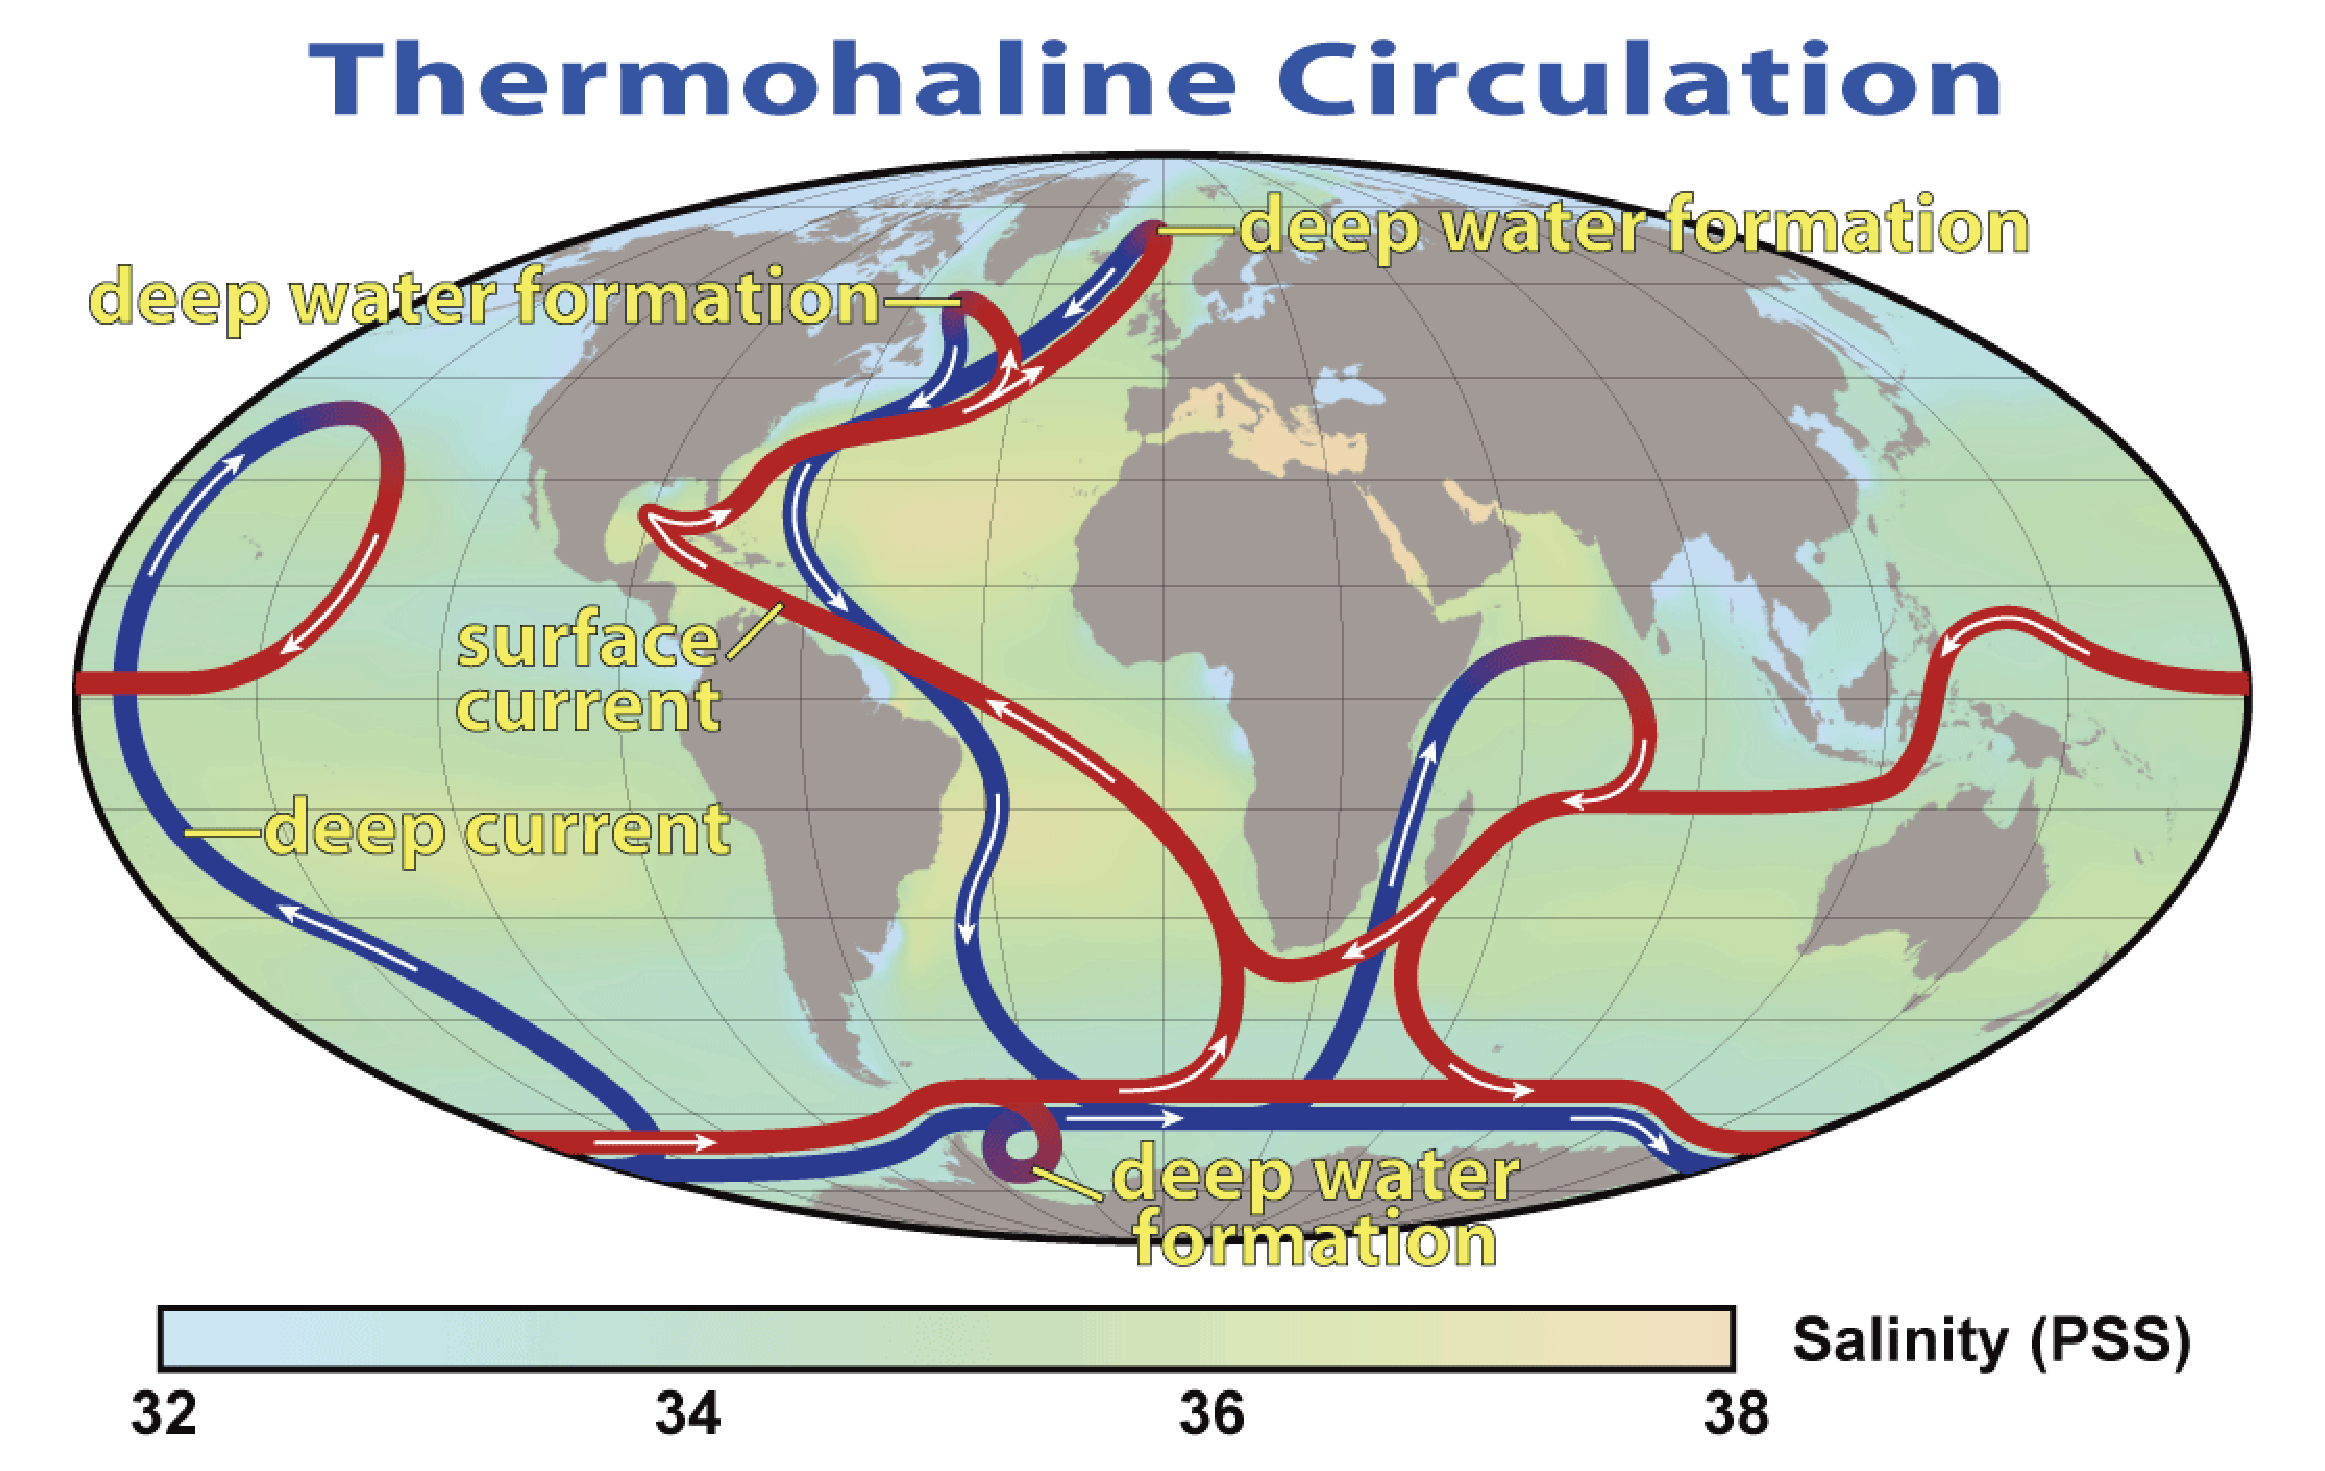
\includegraphics[width=4in]{Images/ConvBelt}
  \caption[Schematic of meridional overturning circulation]{Schematic of meridional overturning circulation.  The lighter arrows represent surface currents and darker arrows represent deep water currents.  \cite{Wiki}}\label{f:ConvBelt}
\end{figure}
\end{center}

As was mentioned earlier, the ocean can be described in 4 distinct layers.  Figure \protect \ref{f:OceCol} shows the four layers: the mixed layer, seasonal thermocline, main thermocline, and the abyssal layer.  The top 10 meters of the ocean is called the mixed layer, which gets its name due to the stirring by the wind.  The mixed layer is not stratified and therefore density is approximately constant in the vertical direction.  The next layer down, the seasonal thermocline, is about 100 m of depth.  It is seasonal because the stratification in the seasonal thermocline is erased every winter by convection.  Below it, the main thermocline, which varies from about 500-1000 m of depth, is permanently stratified.  Below that, is the rest of the ocean, which is called the abyssal layer.  The main thermocline and the abyssal layer make up what is known as the ocean interior.

\begin{center}
\begin{figure}[h!]
\centering
  % Requires \usepackage{graphicx}
  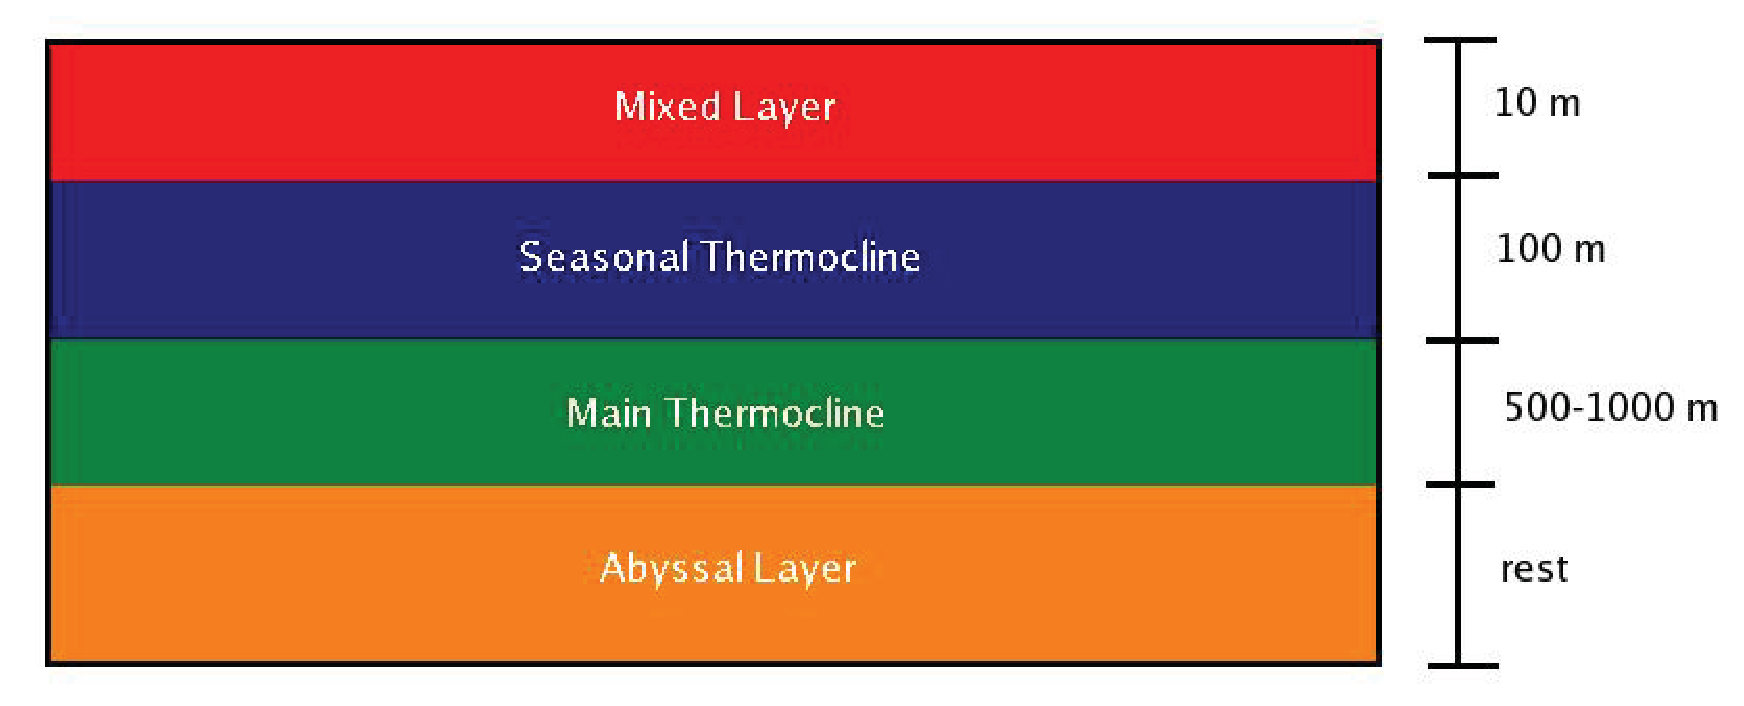
\includegraphics[width=4in]{Images/OceanColumn}
  \caption[Diagram of Ocean Column]{Diagram of Ocean Column.  Oceans are typically about 5 km deep.}\label{f:OceCol}
\end{figure}
\end{center}

\subsection{Ocean Phenomena and Their Scales of Motion}

One of the difficulties that comes with modeling the ocean is how to incorporate and accurately model the immense range of spatial and temporal scales.  The scales range from small scale turbulence that one can see instantaneously when the waves splash up on the beach all the way up the largest scale gyres such as the MOC that cover the entire global ocean and take decades to complete one full cycle.  Table \protect \ref{t:scales} lists ocean phenomena and the scales of motion associated with them.

\begin{center}
\begin{table}[h!]
\begin{tabular}{|c|c|c|c|}
\hline
\textbf{Ocean Phenomenon} & \textbf{L}  &   \textbf{U}  & \textbf{T}  \\
\hline
Microturbulence   & 1-100 cm & 1-10 cm/s & 10-100 s \\

Internal Gravity Waves   & 1-20 km & 0.05-0.5 m/s & min-hrs\\

Tides   & Basin Scale & 1-100 m/s & Hours\\

Coastel Upwelling   & 1-10 km & 0.1-1 m/s & several days\\

Mesoscale Eddies   & 5-500 km & 0.1-1 m/s & Days to Months\\

Rossby Waves & Basin Scale & 0.5-2 m/s & Months to Years\\

Major Currents & 50-500 km & 0.5-2 m/s & Weeks to Seasons\\

Large-scale Gyres  & Basin Scale & 0.01-0.1 m/s & Decades and Beyond\\
\hline
\end{tabular} \\[1ex]
\caption[Scales of ocean phenomenon]{List of Ocean phenomenon and their associated scales. \cite{94CushRoi}}
\label{t:scales}
\end{table}
\end{center}

Microturbulence occurs in the top layer of the ocean (the mixed layer).  This is small scale turbulence that occurs due temperature and salinity variations that exist in the mixed layer being disturbed by the wind.  This small scale phenomenon is often modeled using different turbulence parameterization in large ocean general circulation models.

IGravity waves occur both on the surface and on the interior of the ocean.  Gravity waves occur at the interface of two fluids with different densities.  Surface gravity waves are easily seen in the ocean, especially on the coast.  There is a disturbance that causes the water to be displaced upwards.  Then, the water that has been raised is heavier than the air around it and it is naturally pulled back down by gravity.  The inertia from the vertical velocity that has developed causes the fluid to then penetrate the surface below the equilibrium level.  This process repeats causing oscillations along the surface that make up the waves.  The waves travel becuase of the change in the phase of the oscillations from place to place.  The same phenomenon happens in the interior of the ocean between two different layers of stratified flow.  These waves are slower and longer, since the density difference is much smaller.

Tides are caused by the forces of the moon and the sun acting on the ocean.  This causes the rising and falling of the ocean's surface.  The distance between the earth and Moon is shorter than the earth and Sun, so the effect of the lunar tides is greater (about twice as great compared to solar tides).  As seen in Figure \protect \ref{f:Tides}, a high tide occurs when the moon aligns with a section of the earth.  The effect of the moon's gravity pulling on the earth, raises the ocean level in the region nearest the moon.  Also, since the earth is being pulled more than the ocean waters on the opposite side of the earth, that side also "rises".  The low tide occurs normal to that location in either direction, due to conservation of mass.  This explains semidaily or semidiurnal tides, which have two high tides and two low tides each day.  However, there are also daily/diurnal tides, which have one low and one high tide per day.

\begin{center}
\begin{figure}[h!]
\centering
  % Requires \usepackage{graphicx}
  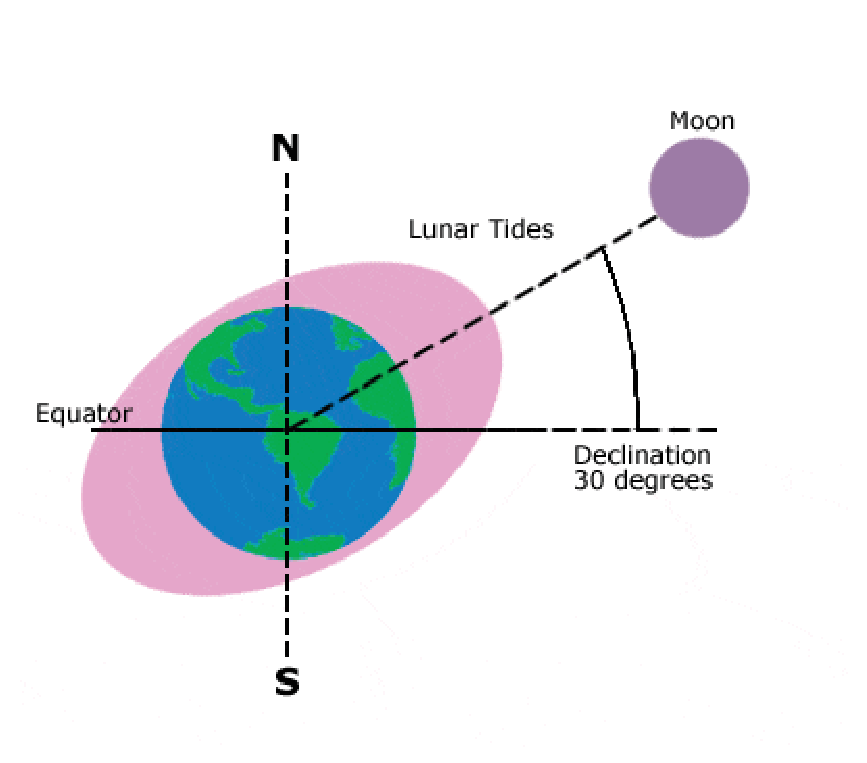
\includegraphics[width=4in]{Images/tidal}
  \caption[Exaggerated schematic of tides]{Exaggerated schematic of tides.  \cite{tides}}\label{f:Tides}
\end{figure}
\end{center}

Upwelling occurs in many ways in the ocean.   There is upwelling at the coast, in the interior, near the equator.  Upwelling occurs when wind-driven warm, surface water is moved and replaced by deep, cold water.  In the Northern Hemisphere, wind-driven currents are diverted to the right of the wind direction (in the Southern Hemisphere they are diverted to the left due to the Coriolis effect).  This is known as Ekman transport (a balance of the Coriolis effect and friction).  And by the coast, when the wind aligns with the coast on its left, the Ekman transport will move the ocean water to the right (in the Northern Hemisphere), see Figure \ref{f:upwelling}.  This removes warm, nutrient-lacking water and replaces it with cold, nutrient-rich water.  This is especially important for the oceanic food chain and for fisheries.  

\begin{center}
\begin{figure}[h!]
\centering
  % Requires \usepackage{graphicx}
  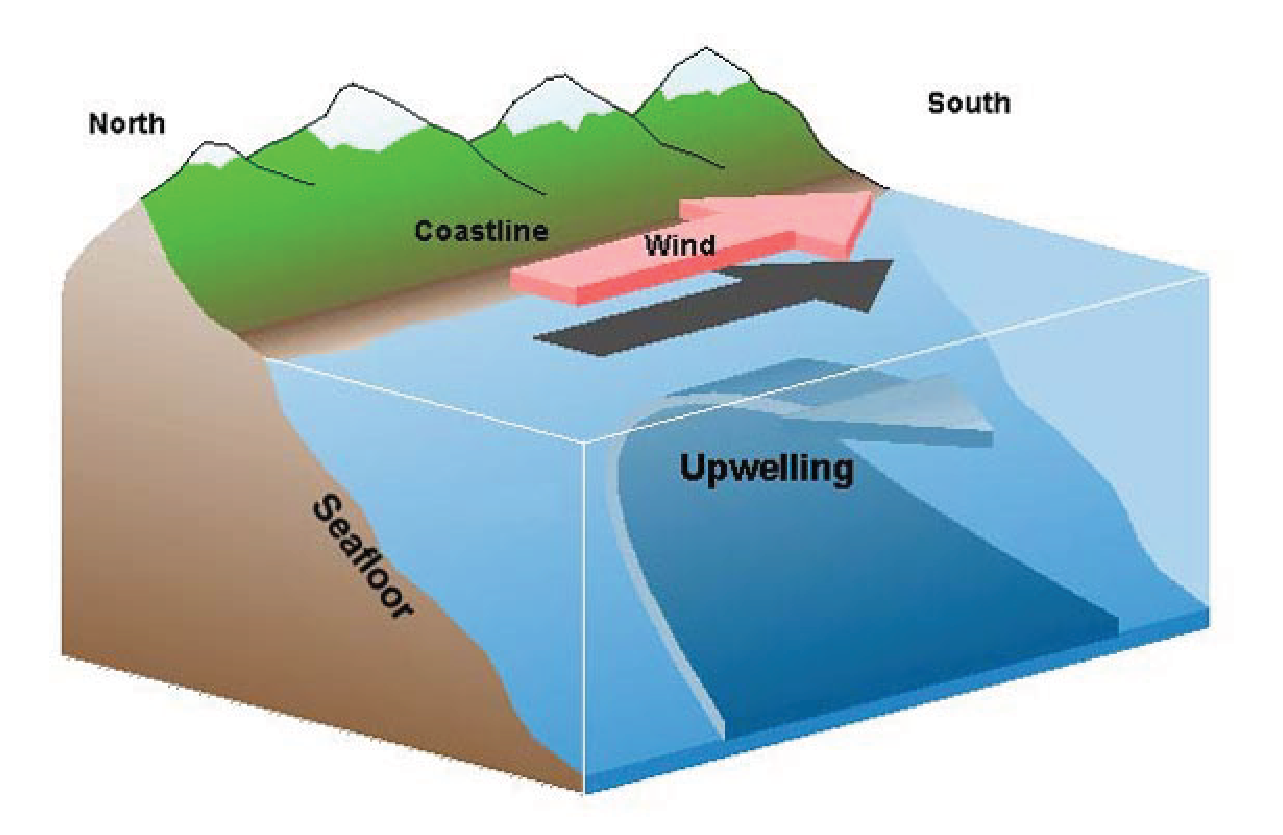
\includegraphics[width=4in]{Images/Upwelling}
  \caption[Coastal Upwelling]{A schematic of coastal upwelling. \cite{Wiki}}\label{f:upwelling}
\end{figure}
\end{center}
%Wikipedia

Eddies have a vast range of scales in the ocean.  The eddies of interest in oceanography are referred to as mesoscale eddies and typical values in the ocean are listed in the Table \ref{t:scales}.  These eddies are typically formed when an ocean current has an instability.  This instability eventually grows enough to detach from the large current.  These mesoscale eddies are typically formed of water masses that are different from the surrounding water.  The circulation in this eddy can be quite fast and of concern for the various operations at sea.  It also contributes to the transport of heat within the ocean.  Figure \ref{f:eddies} shows a picture of a mesoscale eddy that formed when the Oyashio and Kuroshio currents collided.  

\begin{center}
\begin{figure}[h!]
\centering
  % Requires \usepackage{graphicx}
  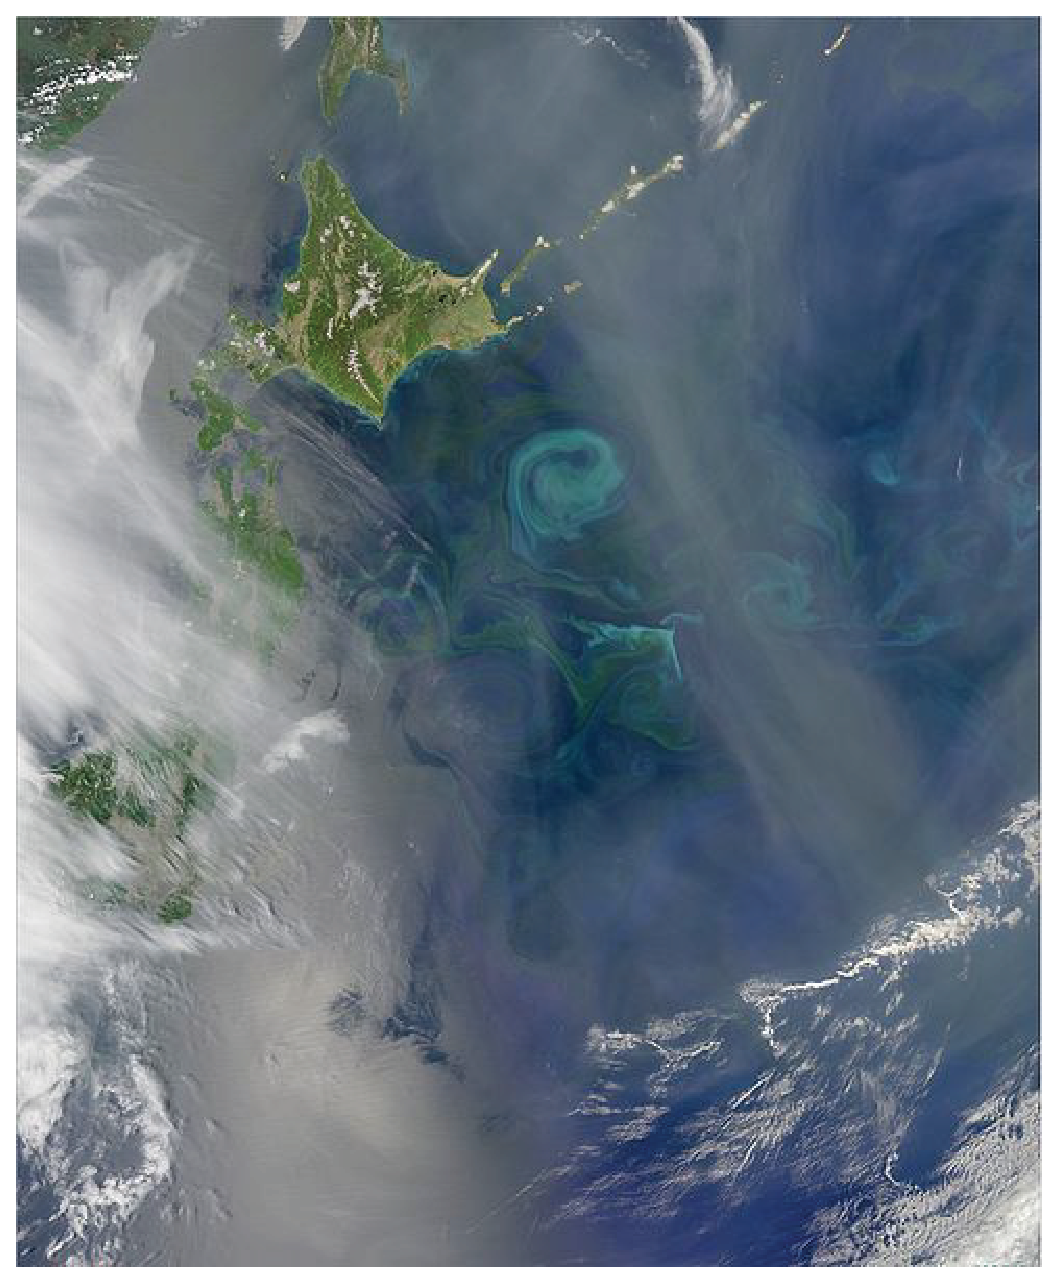
\includegraphics[width=4in]{Images/eddies}
  \caption[Mesoscale Eddies]{The Oyashio and Kuroshio currents collide and a mesoscale eddy is created.  In this picture, the phytoplankton bcome concentrated along the boundary of the eddy and it traces out its motion.  \cite{Wiki}}\label{f:eddies}
\end{figure}
\end{center}
%Wikipedia

Rossby waves a large scale waves that can affect large ocean currents.  These waves are prompted by the meridional change in the Coriolis parameter.  These small variations in the Coriolis parmeter turn a steady, geostrophic flow into a sowly moving planetary waves.  These waves are very difficult to see in the real ocean.  

Major ocean currents are large scales circulations.  The most well-known example is the Gulf Stream and Kuroshio currents.

\begin{center}
\begin{figure}[h!]
\centering
  % Requires \usepackage{graphicx}
  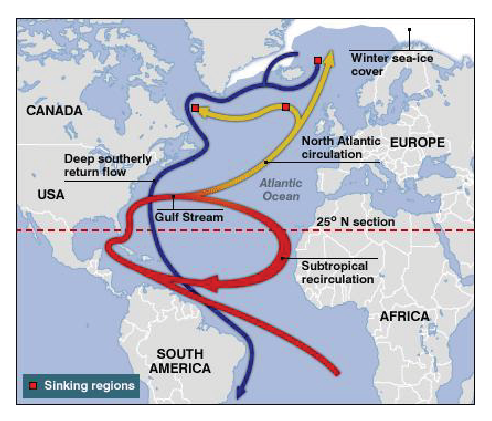
\includegraphics[width=2in]{Images/GulfStream}
  \caption[Gulf Stream]{Circulation patterns of Gulf Stream. \cite{Wiki}}\label{f:GulfStream}
\end{figure}
\end{center}
%Wikipedia

Large-scale gyres is referring to circulations like the thermohaline circulation.

\section{Derivation of Governing Equations}
\label{derivegoverningeqns}

In this section, a review of three sets of governing equations that describe ocean circulation will be derived.  These include the non-hydrostatic primitive equations, the hydrostatic primitive equations, and shallow water equations, which are in order from most general to the most simplified.  \cite{94CushRoi}

\subsection{Primitive Equations (Non-hydrostatic Primitive Equations)}

As discussed earlier, the difference between geophysical flows versus most engineering flows, is that geophysical flows are affected by the rotation of the earth.  Therefore, the governing equations need to incorporate the effect of the earth's rotation.  This is done by transforming from the inertial frame of reference where Newton's second law is valid into a rotating frame of reference (of the earth).  The result from this transformation is the addition of fictitious forces (Coriolis and centrifugal).  The centrifugal force only slightly distorts the earth, because gravity far exceeds the centrifugal force, so it is usually just absorbed into the gravity term.  The Coriolis force is not negligible.  Taking a time derivative with respect to the inertial framework is equivalent to applying the following operator, 
%
\begin{equation*}\label{e:coriolisoperator}
\frac{D}{Dt} + 2 {\bf \Omega}  \times
\end{equation*}
%
in a rotating framework (ignoring centrifugal component), where ${\bf \Omega} = \Omega {\rm cos} \phi {\bf j} + \Omega {\rm sin} \phi {\bf k}$ is a vector of the angular rotation of the earth and $\phi$ is latitude.  This results in the following components, 
%
\begin{equation*}\label{e:accelx}
\frac{Du}{Dt} + 2 \Omega {\rm cos} (\phi) w - 2 \Omega {\rm sin} (\phi) v
\end{equation*}
\begin{equation*}\label{e:accely}
\frac{Dv}{Dt} + 2 \Omega {\rm sin} (\phi) u
\end{equation*}
\begin{equation*}\label{e:accelz}
\frac{Dw}{dt} - 2 \Omega {\rm cos} (\phi) u
\end{equation*}
%
where often the quantities are defined as, $f = 2 \Omega {\rm sin} (\phi)$ and $f_{*} = 2 \Omega {\rm cos} (\phi)$.  The coefficient,  $f$, is the Coriolis parameter and the $f_{*}$ is the reciprocal Coriolis parameter.  The Coriolis parameter is positive in the Northern Hemisphere, negative in the Southern Hemisphere and zero at the equator.  The reciprocal Coriolis terms are typically neglected because they are much smaller than the Coriolis terms.  Making these adjustments for a rotating framework to the Navier-Stokes equations for a Newtonian fluid gives, 
%
\begin{equation}\label{e:NSrotating}
\rho \left( \frac{D {\bf u}}{D t} + f \hat{\bf k} \times {\bf u} \right)= -\nabla P - \rho g \hat{\bf k} + \mu \nabla ^2 {\bf u} 
\end{equation}
%
where $\rho$ is density, $p$ is pressure, $g$ is gravitational acceleration, $\mu$ is dynamic viscosity.  Also, $\frac{D}{Dt}$ is the total derivative.  The x-, y- and z- are aligned with the local east, north and up directions.  Since the ocean follows the curvature of the earth, a curvilinear coordinate system is the most accurate way to describe the ocean's fluid motion.  In that case, Equation \ref{e:NSrotating}, becomes, 
%
\begin{equation}\label{e:xmomc}
    \rho \left ( \frac{Du}{Dt}  -\frac{uv \tan \phi}{r} + \frac{uw}{r}  - f v \right ) = - \frac{\partial p}{\partial x} + F_x
\end{equation}

\begin{equation}\label{e:ymomc}
    \rho \left ( \frac{Dv}{Dt} + \frac{u^2 \tan \phi}{r}+\frac{uw}{r}+fu \right ) = - \frac{\partial p}{\partial y} + F_y
\end{equation}

\begin{equation}\label{e:zmomc}
    \rho \left ( \frac{Dw}{Dt} - \frac{u^2+v^2}{r} \right) = - \frac{\partial p}{\partial z}-\rho g + F_z
\end{equation}
%
where, $\phi$ is latitude and r is the distance to the center of the earth.  $F_x$, $F_y$, and $F_z$ represent the viscous forces, which are slightly more complicated with the addition of the curvilinear terms.  However, in ocean modeling, the length scales are typically restricted to something substantially shorter than the radius of the earth.  As a result, all the additional curvilinear terms can be neglected (including those in the viscous term).  Thus, Equation \ref{e:NSrotating} is used.  This assumption can be thought of as the distortion introduced when mapping the curved earth's surface on to a flat plane.  

In addition to momentum, the primitive equations include conservation of mass, 
%
\begin{equation}\label{e:conto}
    \frac{\partial \rho}{\partial t} + \nabla \cdot (\rho {\bf u})
\end{equation}
%
As mentioned before, one of defining features of geophysical flows is the role of stratification.  This feature is incorporated through the density field.  The density in the ocean mainly depends on the local temperature, $T$ and salinity, $S$.  The warmer the temperature, the less density the water.  And the saltier the water is more dense.  Therefore, the equation of state for seawater has some dependence on these two quantities, and as a rough approximation, this could be some linear relationship, 
%
\begin{equation}\label{e:eqst}
    \rho = \rho_0 [1 - \alpha(T-T_0) + \beta(S - S_0) ]
\end{equation}
%
The constants $\rho_0, T_0, S_0$ are reference values and $\alpha$ and $\beta$ are the coefficient of thermal expansion and the coefficient of saline contraction, respectively.  Thus, the primitive equations often include some energy equations, mainly in the form of temperature and salinity budgets,
%
\begin{equation*}\label{e:eneroo}
    \rho C_\nu \frac{dT}{dt}+p \left ( \nabla \cdot {\bf u} \right ) = k \nabla^2 T
\end{equation*}

\begin{equation*}\label{e:salt}
    \frac{dS}{dt} = \kappa_S \nabla^2 S
\end{equation*}
%
where $C_{\nu}$ is the heat capacity at constant volume, $k$ is thermal conductivity of seawater, and $\kappa_S$ is the coefficient of salt diffusion.  

In the ocean, the fluid density does not vary greatly.  The relative density difference is usually less than 2 \% \cite{94CushRoi}.  Therefore, one can write the density in terms of a mean component and a fluctuating component,
%
\begin{equation}\label{e:den}
    \rho = \rho_0 + \rho ' (x, y, z, t)
\end{equation}
%
where $\rho ' \ll \rho_0$.  $\rho '$ is the fluctuation due to stratification and the motion of the fluid, which is small compared to the reference value, $\rho_0$.  This approximation is called the Boussinesq approximation.  If Equation \ref{e:den} is plugged into the continuity equation, Equation \protect \ref{e:conto}, scale analysis results in the following equation, 
%
\begin{equation}\label{e:cont}
    \nabla \cdot {\bf u} = 0
\end{equation}
%
This new divergence-free requirement means the volume is conserved.  This also eliminates sound waves.

Next, the x and y momentum equation, can be similarly treated.  Equations \protect \ref{e:xmomc} and \protect \ref{e:ymomc} have a $\rho$ on the far left side.  Ignoring the density variation component ($\rho '$), the $\rho$ can be replaced by the mean value $\rho_0$.  This leaves equations \protect \ref{e:xmoms} and \protect \ref{e:ymoms}.
%
\begin{equation}\label{e:xmoms}
     \frac{Du}{Dt} - fv = - \frac{1}{\rho_0} \frac{\partial p}{\partial x} + \nu \nabla^2 u
\end{equation}

\begin{equation}\label{e:ymoms}
     \frac{Dv}{Dt}+fu = - \frac{1}{\rho_0} \frac{\partial p}{\partial y} + \nu \nabla^2 v
\end{equation}
%
The z-momentum equation (Equation \protect \ref{e:zmomc}) has a $\rho$ not only on the far left side but also in the product with g on the right side.  The left side can be treated the same as the x and y momentum equations.  The term $\rho g$ accounts for the weight of the fluid which affects the pressure.  Writing presure analogous to how the density was written, 
%
\begin{equation*}
    p=p_0(z)+p'(x, y, z, t)
\end{equation*}
%
In the ocean, the pressure is often assumed hydrostatic, which means it only varies with depth.  In this case, a less strict assumption is to assume that the reference pressure is hydrostatic, 
%
\begin{equation}\label{e:pres}
    p_0(z)=P_0 - \rho_o gz
\end{equation}
%
This means that $\frac{dp_0}{dz}=-\rho_0 g$ and when all is substituted into the Equation \protect \ref{e:zmomc}, it reduces to, 
%
\begin{equation}\label{e:zmoms}
    \frac{Dw}{Dt} = -\frac{1}{\rho_0} \frac{\partial p'}{\partial z} - \frac{\rho ' g}{\rho_0} + \nu \nabla^2 w
\end{equation}
%
The energy equation (Equation \protect \ref{e:eneroo}) can first be simplified by removing the second term due to the conservation of volume (Equation \protect \ref{e:cont}).  As was done in all the momentum equations, the $\rho$ term on the left side can be replaced with $\rho_0$.  Then, the energy equation reduces to Equation \protect \ref{e:eners}.
%
\begin{equation}\label{e:eners}
    \frac{dT}{dt} = \kappa_T \nabla^2 T
\end{equation}
%
where $\kappa_T = \frac{k}{\rho_0 C_\nu}$.  Due to the similarity between the temperature equation and the salinity equation (Equation \protect \ref{e:salt}), these two equations can be combined to determine the evolution of density.  However, the simplification can only be made if diffusion is not primarily governed by molecular processes.  Therefore, this is only the case on small scales.  In general, it can be assumed that in turbulence, diffusion is accomplished by eddies, which mix the salt and heat at equal rates.  If this is the case, the terms $\kappa_S$ and $\kappa_T$ are equal, thus, $\kappa_S=\kappa_T=\kappa$, also known as the eddy diffusivity.  By combining equations \protect \ref{e:salt}, \protect \ref{e:eners} and \protect \ref{e:eqst}, the energy equation becomes the density equation (Equation \protect \ref{e:densf}).
%
\begin{equation}\label{e:densf}
    \frac{D \rho '}{dt} = \kappa \nabla ^2 \rho '
\end{equation}
%
Now, that there are no longer any terms $\rho$ and p, the primes on $\rho '$ and p' are usually dropped throughout all the equations.  The above simplifications make up the Boussinesq approximation.

To summarize, the Boussinesq approximation results in the following non-hydrostatic primitive equations.
%
\begin{equation}\label{e:xmom_nh}
    \frac{D {\bf u}}{Dt} + f  \hat{\bf k} \times {\bf u}= - \frac{1}{\rho_0} \nabla p + \frac{\rho g}{\rho_0} \hat{\bf k} + \nu \nabla^{2} {\bf u}
\end{equation}

\begin{equation}\label{e:cont_nh}
   \nabla \cdot {\bf u} = 0
\end{equation}

\begin{equation}\label{e:ener_nh}
   \frac{D \rho}{dt} = \kappa \nabla ^2 \rho
\end{equation}

\subsection{Hydrostatic Primitive Equations}

\begin{center}
\begin{table}
\centering
\begin{tabular}{|c|c|c|c|}
\hline
\textbf{Variable} & \textbf{Scale}  &   \textbf{Unit}  & \textbf{Value}  \\
\hline
x & L & m & 10 km = $10^4$ m \\

y & L & m & 10 km = $10^4$ m \\

z & H & m & 100 m \\

u & U & m/s & $\geq$ 1 day $\simeq 9 x 10^4$ s \\

v & U & m/s & $\geq$ 1 day $\simeq 9 x 10^4$ s \\

w & W & m/s &  \\

p & P & $kg/ms^2$ & \\

$\rho$ & $\delta \rho$ & $kg/m^3$ & 0.1 \% of $\rho_0$ \\

\hline
\end{tabular} \\[1ex]
\caption[Typical ocean scales]{Typical Ocean Scales.  \cite{94CushRoi}}
\label{t:scales2}
\end{table}
\end{center}

In most ocean models, the primitive equations are taken one step further by simplifying them with some scale analysis.  Table \protect \ref{t:scales2} summarizes the scales associated with the different ocean variables.  As shown in this table, the horizontal lengths and velocities are equivalent in terms of scales, while the vertical is different.  The ocean domain is much wider than it is tall.  The ocean currents are generally confined to the upper hundred meters, but can extend horizontal in both directions over tens of kilometers.  The approximation, then, is that $H \ll L$.  The velocity scales will also be different and a look at the continuity equation can give that relationship, 
%
\begin{align*}
\quad \qquad \frac{\partial u}{\partial x}  \quad +  \quad    \frac{\partial v}{\partial y}  \quad    +    \quad  \frac{\partial w}{\partial z} \quad = \quad 0\\
{\rm O}\left(\frac{U}{L}\right) \quad {\rm O}\left(\frac{U}{L}\right) \quad {\rm O}\left(\frac{W}{H}\right) \qquad 
\end{align*}
%
The last term, $\frac{\partial w}{\partial z}$, cannot be greater than the other two terms because that would mean the equation would reduce to $\frac{\partial w}{\partial z}=0$, which isn't a good approximation for everywhere in the ocean.  Since at the bottom of the ocean, the vertical direction of the flow is going to need to converge laterally when it hits the bottom surface.  Therefore, the order of the last term needs to be less than or equal to the order of the other two terms. This gives the following relationship:
%
\[W \leq \frac{H}{L} U\]
%
and since $H \ll L$, then, $W \ll U$.  If a scale analysis using these two simplifications is done on the non-hydrostitic momentum equations (Equation \ref{e:xmom_nh}), the equations reduce to Equations \protect \ref{e:mom_hpe} - \ref{e:zmom_hpe}.  This scale analysis simplifies the z momentum equation and it becomes the hydrostatic pressure approximation.  Therefore, the equations that result from this scale analysis are known as the hydrostatic primitive equations.  

Lastly, the density equation, Equation \ref{e:ener_nh}, can only be simplified by its diffusion term.  The horizontal diffusion drops out and the resulting equation is Equation \protect \ref{ener}.

To summarize, the Boussinesq approximation and scale analysis results in the following hydrostatic primitive equations,
%
\begin{equation}\label{e:mom_hpe}
    \frac{\partial {\bf u_h}}{\partial t} + {\bf u} \cdot \nabla {\bf u_h} + f  \hat{\bf k} \times {\bf u_h}= - \frac{1}{\rho_0} \nabla_h p +  \nu \nabla^{2} {\bf u_h}
\end{equation}

\begin{equation}\label{e:zmom_hpe}
    0 = - \frac{\partial p}{\partial z} - \rho g
\end{equation}

\begin{equation}\label{e:cont_hpe}
   \frac{\partial w}{\partial z} = - \nabla_{h}{\bf u}_{h} 
\end{equation}

\begin{equation}\label{e:ener_hpe}
   \frac{D \rho}{D t}  = \kappa \frac{\partial^2 \rho}{\partial z^2}
\end{equation}
where ${\bf u_h}$ is the horizontal velocity components $u$ and $v$.  

\subsection{Shallow Water Model}

The shallow water model is a simplified model of the ocean commonly used to look at large scale ocean circulation patterns.  There are numerous applications where the horizontal length scale is much larger than the vertical length scale and thus, these equations are quite useful.  They have been used for solving various oceanic \cite{07BCLDR, 04BILH}, atmospheric problems as well as dam breaking \cite{06RSS, 02bSZ} and river flow problems \cite{94Vreug}.  

The shallow water model can be derived from the hydrostatic primitive equations (Equations \ref{e:mom_hpe} - \ref{e:ener_hpe}).  Assuming that the flow is homogeneous (no stratification) and frictionless, the equations become, 
%
\begin{equation}\label{e:mom_temp}
    \ \frac{\partial {\bf u_h}}{\partial t} + {\bf u} \cdot \nabla {\bf u_h}   + f  \hat{\bf k} \times {\bf u_h}= - \frac{1}{\rho_0} \nabla_h p 
\end{equation}

\begin{equation}\label{e:zmom_temp}
    0 = - \frac{\partial p}{\partial z} 
\end{equation}

\begin{equation}\label{e:cont_temp}
    \nabla \cdot {\bf u} = 0
\end{equation}
%
Assuming that the horizontal flow field is initially independent of depth, then it will remain independent of depth at future times.  Also, the pressure is independent of $z$ because of Equation \ref{e:zmom_temp}.  Since all the advection terms, the Coriolis terms and the pressure terms are all independent of z, that means $u$ and $v$ will remain z-independent at all times.  In geophysical fluid dynamics, flows under this assumption are called barotropic.   Thus, the x and y momentum equations reduce to, 
%
\begin{equation}\label{e:mom_temp1}
    \ \frac{\partial {\bf u_h}}{\partial t} + {\bf u_h} \cdot \nabla {\bf u_h}   + f  \hat{\bf k} \times {\bf u_h}= - \frac{1}{\rho_0} \nabla_h p 
\end{equation}
%
where the subscript $h$ can be dropped.  Now, since the velocities are homogeneous in the z direction (or depth averaged), the same needs to be done to the continuity equation, Equation \ref{e:cont_temp}.  The first two terms are independent of z, but a vertical velocity varying with depth can exist.  Integrate Equation \ref{e:cont_temp} over the entire fluid depth will give, 
%
\begin{equation}\label{e:integ_cont}
    (\frac{\partial u}{\partial x} + \frac{\partial v}{\partial y}) \int^{b+\eta}_{b} dz + [w]_{b}^{b+\eta} = 0
\end{equation}
%
where $b$ is a function describing the spatially varying bottom bathymetry and $\eta$ is the sea surface height.  For boundary conditions, the vertical velocity has to obey the following properties at the surface and bottom boundaries (particles on surface cannot leave surface, particles on the bottom cannot leave bottom), 
%
\begin{equation*}
    w(z=b+\eta) = \frac{\partial (b + \eta)}{\partial t} + u \frac{\partial (b+ \eta)}{\partial x} + v \frac{\partial (b+\eta)}{\partial y}
\end{equation*}

\begin{equation*}
    w(z=b) = \frac{\partial b}{\partial t} + u \frac{\partial b}{\partial x} + v \frac{\partial b}{\partial y}
\end{equation*}
therefore, Equation \ref{e:integ_cont} becomes, 
\begin{equation*}
    \frac{\partial \eta}{\partial t} + \frac{\partial (\eta u)}{\partial x} + \frac{\partial (\eta v)}{\partial y} =0
\end{equation*}
%
This replaces the continuity equation and eliminates vertical velocity from the formulation.  Dynamic pressure can also be calculated, it is homogeneous and independent of depth (assuming uniform atmospheric pressure over the ocean).  This is, 
%
\begin{equation*}
   p=\rho_{0} g (\eta +b)
\end{equation*}
%
This pressure can be substituted into the momentum equations (Equation \ref{e:mom_temp1} )and closes the problem with three equations and three unknowns.  For a flat bottom ($b(x, y)$ does not vary spatially), the shallow water equations are
%
\begin{equation}\label{e:swe_xmom}
    \frac{\partial u}{\partial t} + u \frac{\partial u}{\partial x} + v \frac{\partial u}{\partial y} - fv = - \frac{1}{\rho_0} \frac{\partial \eta}{\partial x} 
\end{equation}

\begin{equation}\label{e:swe_ymom}
    \frac{\partial v}{\partial t} + u \frac{\partial v}{\partial x} + v \frac{\partial v}{\partial y} + fu = - \frac{1}{\rho_0} \frac{\partial \eta}{\partial y}
\end{equation}

\begin{equation}\label{e:swe_cont}
    \frac{\partial \eta}{\partial t} + \frac{\partial (\eta u)}{\partial x} + \frac{\partial (\eta v)}{\partial y}=0
\end{equation}

In this work, all three sets of equations have been investigated to see which worked best with the wavelet method and Brinkman penalization.  In the following chapters, the use equations will be further described and results will be discussed.  In the following section, an overview of how current ocean models solve these governing equations.  

\section{Ocean Circulation Modeling}
\label{sec:BackOceanModeling}

There is an exhaustive list of ocean models used in scientific research \cite{oceanmodels}.  Many of the large OGCMs, such as the ones used for climate prediction, have fixed spatial resolution \cite{97JCCGMSTW, 00FBLMRRW, 00GCSBGJMW, 00PGRS, 93GMB, 93GMBD, 96RABCCDEGSS}.  However, there has been some initial progress made on the use of non-uniform grids, as well as adaptive grids.  There are also various techniques that have been developed to handle the complex geometry that is inherit in ocean boundaries and bathymetry.  These models and techniques will be reviewed below.  

The current standard in the majority of ocean models is to use structured meshes \cite{06CBBBB}, typically used with a finite difference method.  A structured mesh is one that has a uniform topological structure, which means if one is given a node, they can determine implicitly what other nodes are connected to it.  Thus, the topology of the mesh is uniform in space.  Therefore, these meshes have a block structure, so that different structured meshes can be used and combined along the interface.  This allows for higher resolution in certain regions of interest.  This is known as a nested grid, which assumes that one knows a priori the location that refinement is needed as well as how much extra resolution is necessary.  Some examples of this include Regional Ocean Modeling System (ROMS) \cite{05SM}, which is a free-surface, terrain-following, hydrostatic primitive equation ocean model.  There is also \cite{96LAM, 99LL}. 
%http://www.myroms.org/

Vertical grids also traditionally use a structured mesh but there are three main choices for the vertical coordinate, as shown in Figure \ref{f:3Regimes}.  The simplest and oldest is the z-coordinate model, which is when the vertical grid is aligned with surfaces of constant depth.  The issue with using the z-coordinate is the difficulty in representing complex bathymetry without introducing sharp corners due to stair-step representation.  A popular alternative is to employ partial cell or shaved cell, as shown in Figure \ref{f:BotTopo}.  These techniques were used successfully by \cite{97AHM}.  

The other vertical coordinates include the $\sigma$-coordinate and isopycnal-coordinate models.  The $\sigma$-coordinate conforms to both the bathymetry and the free surface.  The isopycnal-coordinate model aligns with the surfaces of constant density.  The biggest problem with the $\sigma$-coordinate is that there are substantial errors in the calculation of the horizontal pressure gradient \cite{98MOE}.  The other big problem with the $\sigma$-coordinate model is that the number of vertical levels is held constant over the entire domain.  More details can be found in \cite{99HB}.  

There also exists a hybrid vertical coordinate model, which was developed to fix the issue with the constant vertical levels in the $\sigma$-coordinate model.  This model uses the $\sigma$-coordinates in the shallow regions, z-coordinates in the mixed layer and unstratified regions and isopycnal coordinates in the stratified regions \cite{00GBBCGHHTW, 03CSHB}.  This model tries to take advantage of where each choice of vertical coordinate naturally behaves best.

\begin{center}
\begin{figure}[h!]
\centering
  % Requires \usepackage{graphicx}
  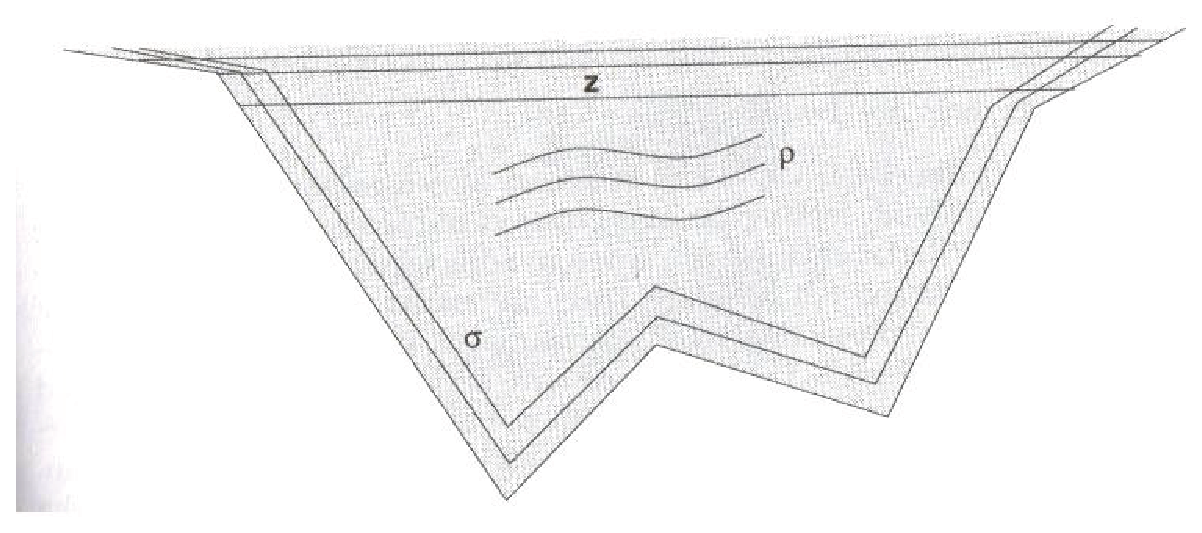
\includegraphics[width=4in]{Images/3Regimes}
  \caption[Vertical coordinates]{Illustration of three choices for a vertical coordinate.\protect \cite{04Gri}}\label{f:3Regimes}
\end{figure}
\end{center}

\begin{center}
\begin{figure}[h!]
\centering
  % Requires \usepackage{graphicx}
  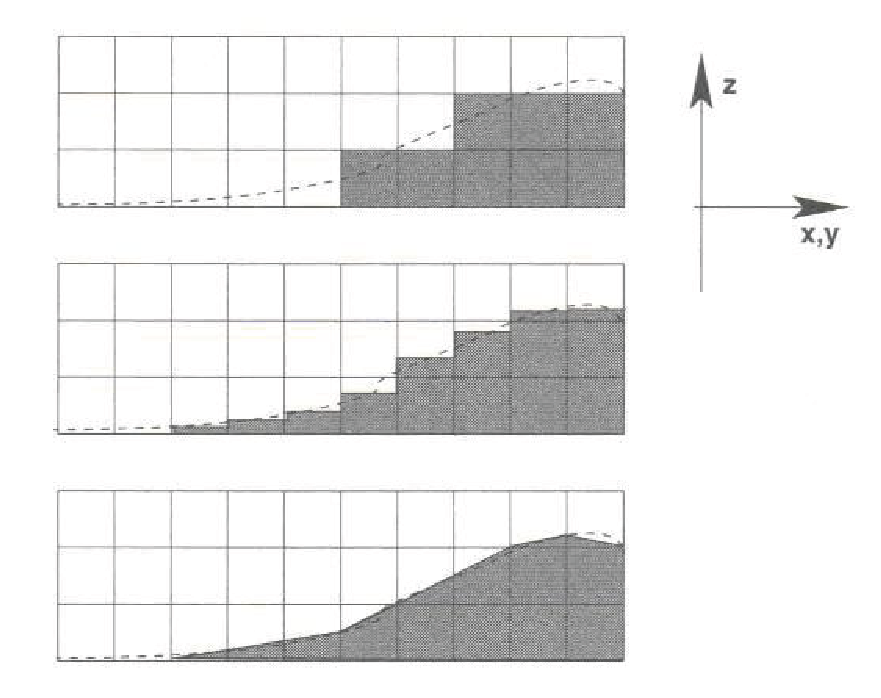
\includegraphics[width=4in]{Images/BotTopo}
  \caption[Z-coordinate options]{Three different representations of bottom topography with the z-coordinate.  The top is called "full cell" and is the oldest, the middle is called "partial cell" and the bottom is called "shaved cell".\protect \cite{04Gri}}\label{f:BotTopo}
\end{figure}
\end{center}

On the other hand, unstructured meshes are less mainstream for ocean models but becoming more popular.  Unstructured meshes allow for an arbitrary mesh structure and are typically solved using finite element, finite volume, and/or spectral methods.  This flexibility allows for a better representation of the coastline and bathymetry.  The use of unstructured meshes is especially prevalent in fields of engineering that work with exterior or interior pipe flow, aircraft wings, etc (some examples include \cite{05MBLP, 97PM, 05ZTZN}).  

The recent review article, \cite{08PPGMK}, gives a extensive overview of what is being done with unstructured adaptive meshes in ocean modeling.  In summary, models with unstructured meshes have been relatively underused over the models with structured meshes in the ocean community.  What follows is a short description of the most well known ocean models using unstructured grids.  

The SUNTANS model from Stanford \cite{06FGS} is also a well-known unstructured-grid model.  In this model, the non-hydrostitic primitive equations are solved using a finite-volume method.  They also use an immersed boundary method to represent the bathymetry.  This is one of the few models that includes the non-hydrostatic dynamics.  

There is also the SEOM \cite{03IHL}, which is a three-dimensional hydrostatic spectral element model with sigma coordinates in the vertical.   The same group has also done some work with the shallow water equations \cite{04BILH}.

The ICOM model from Imperial College which is a non-hydrostatic finite-element model \cite{05PPGFGMEPO, 04FPPGOU, 05GPPOUG, 05PPGPG}.  In this model, they use parallel load-balanced anisotropic adaptive meshes in 3D, so there is no difference in the horizontal and vertical meshes.  

MIT also has a finite-volume, non-hydrostatic ocean model called MITgcm \cite{97MAHPH}.  They did several studies that compared hydrostatic, quasi-hydrostatic and non-hydrostatic, \cite{97MHPA}.  They found that the non-hydrostatic models were just as computational efficient as the hydrostatic models when run in the hydrostatic limit \cite{98MJH}.  

Other unstructured models include the QUODDY finite element 3D hydrostatic model \cite{96LINW}, the FEOM finite element 3D hydrostatic model \cite{04DKS}, the SLIM finite element 3D hydrostatic model \cite{07White}, and FVCOM a finite volume 3D hydrostatic model \cite{03CLB}.  They all do something a little different with the horizontal meshes and with what combination of vertical coordinate and mesh they use.  

Finally, there is an additional topic of mesh adaptivity.  It is clear that having a non-uniform or unstructured mesh is ideal for the majority of ocean simulations.  However, due to the large range of spatial and temporal scales, which are also coupled, the need for a model that can also dynamical adapt on the solution is also beneficial and even necessary for accuracy.  Many processes in ocean modeling are parameterized, but there are many that could easily resolved by having a model that is able to on-the-fly vary its resolution.  \cite{08PPGMK}

There are a few models being used that use mesh adaptivity.  These include both unstructured and structured grids.  The ICOM model is the best example of one using an unstructured grid \cite{05PPGPG, 08PGPACMW, 05PPGFGMEPO}.  Another unstructured mesh optimization algorithm is used by \cite{07BCLDR} uses the shallow water model.  

For structured mesh models, the most common technique is adaptive mesh refinement (AMR).  AMR is similar to the nested grid technique, but much more powerful since there can be many levels of refinement and they can evolve dynamically based on the structure of the solution.  The problem with AMR methods is there are numerical issues with the discrete jumps in resolution.  Some finite difference models that use AMR include \cite{99BD} and \cite{05DBB}.  There is also a finite volume ocean model which uses quadtree refinement, a form of AMR, in the horizontal \cite{07PR}.  


\section{Adaptive Wavelet Collocation Method}
\label{sec:wavelet}

The adaptive mesh numerical technique used is called adaptive wavelet collocation method (AWCM) and was developed by Vasilyev and and collaborators \cite{vasilyev:2003,vasilyev-bowman:2000}.  It is a general method that uses second generation wavelets to efficiently solve partial differential equations.  In this section, we will briefly review this methodology. 

The benefit of using wavelets is that they are localized in both space and time.  They are ideal for use in complex flows where localized structures exist in the solution.  The wavelet collocation method takes advantage of wavelet compression properties.  Functions with localized structures or regions with sharp transitions are well compressed using wavelet decomposition.  This compression is achieved by keeping only the wavelets with coefficients that are greater than an a priori given threshold parameter, thus how the grid adaptation works.  This allows high resolution computations to be carried out only in the regions where it is necessary.  It also allows a solution to be obtained on a near optimal grid for a given accuracy.  

Any function  $u({\bf x})$ in an $n$-dimensional space can be decomposed as \cite{chui:1997,daubechies:1992,mallat:1998}
%Wavelet function decomposition
\begin{equation}
u({\mathbf x})=\sum_{{\mathbf k} \in {\mathcal{K}}^0} c_{\mathbf k}^{0}
\phi_{\mathbf k}^{0}({\mathbf x}) + \sum_{j=0}^{+\infty} \
\sum_{\mu=1}^{2^{n}-1}\ \sum_{{\mathbf l} \in {\mathcal{L}}^{\mu,
j}} d_{\mathbf l}^{\mu, j} \psi_{\mathbf l}^{\mu, j}({\mathbf x})
\label{eq:wavelet-decomp}
\end{equation}
%
where $\phi_{\mathbf k}^{0}(\mathbf x)$ are scaling functions on the lowest level of resolution and $\psi_{\mathbf l}^{\mu, j}({\mathbf x})$ are the wavelet basis functions. Also, $c_{\mathbf k}^{0}$ and $d_{\mathbf l}^{\mu, j}$ are the scaling and wavelet coefficients, respectively. These wavelet coefficients $d_{\mathbf l}^{\mu, j}$ will be small except near areas with large gradients.  Equation \ref{eq:wavelet-decomp} can be decomposed into two terms whose wavelet coefficients are above and below a chosen threshold \mbox{parameter $\epsilon$,}
%
\begin{equation}
u({\mathbf x})=u_{\ge}({\mathbf x}) + u_{<}({\mathbf x}),
\label{eq:wavelet-split}
\end{equation}
%
where
%
\begin{eqnarray}
u_{\ge}({\mathbf x}) &=& \sum_{{\mathbf k} \in {\mathcal{K}}^0} c_{\mathbf
k}^{0} \phi_{\mathbf k}^{0}({\mathbf x}) + \sum_{j=0}^{+\infty} \
\sum_{\mu=1}^{2^{n}-1}\ \sum_{
{ \vspace{-10pt}
        \stackrel{ \mbox{\hspace{5pt}\scriptsize
         ${    {\mathbf l} \in {\mathcal{L}}^{\mu, j}}$ \hspace{5pt}} }{
         \mbox{ \rule[0pt]{0pt}{10pt}\scriptsize%\rulebox used to set spacing above d>eps
         $| d^{\mu, j}_{\mathbf l} | \ge \epsilon \|u \|$} }    
%\begin{array}[t]{c}
%\\*[-2pt]
%\mbox{\scriptsize ${\mathbf l} \in {\mathcal{L}}^{\mu, j}$}
%\\*[-2pt]
%\mbox{\scriptsize $| d^{\mu, j}_{\mathbf l} | \ge \epsilon \|u \|$}
%\end{array}
}}
d_{\mathbf l}^{\mu, j} \psi_{\mathbf l}^{\mu, j}({\mathbf x}) ,
\label{eq:u_ge} \\
u_{<}({\mathbf x}) &=& \sum_{j=0}^{+\infty} \
\sum_{\mu=1}^{2^{n}-1}\ \sum_{
{ \vspace{-10pt}
        \stackrel{ \mbox{\hspace{5pt}\scriptsize
         ${    {\mathbf l} \in {\mathcal{L}}^{\mu, j}}$ \hspace{5pt}} }{
         \mbox{ \rule[0pt]{0pt}{10pt}\scriptsize%\rulebox used to set spacing above d>eps
         $| d^{\mu, j}_{\mathbf l} | < \epsilon \|u \|$} }    
%\begin{array}[t]{c}
%\\*[-2pt]
%\mbox{\scriptsize ${\mathbf l} \in {\mathcal{L}}^{\mu, j}$}
%\\*[-2pt]
%\mbox{\scriptsize $| d^{\mu, j}_{\mathbf l} | < \epsilon \|u \|$}
%\end{array}
}}
d_{\mathbf l}^{\mu, j} \psi_{\mathbf l}^{\mu, j}({\mathbf x}) ,
\label{eq:u_lt}
\end{eqnarray}
%
Donoho \cite{donoho:1992} was able to show that for a regular
function the error is bounded as
%
\begin{equation}
\| u({\mathbf x})-u_{\ge}({\mathbf x}) \|  \le C_1 \epsilon \|u \|
\label{eq:conv_eps},
\end{equation}
%
which means that the number of grid points needed to solve a numerical problem can be significantly reduced while still retaining a prescribed level of accuracy determined by the threshold parameter $\epsilon$.

In the wavelet collocation method there is a one-to-one correspondence between grid points and wavelets. Thus, this makes calculation of nonlinear terms simple, and allows the grid to adapt automatically to the solution at each time step by adding or removing wavelets.  In addition to the points with high enough wavelet coefficients, there are several other checks done to make sure the resolution is sufficient for the given simulation.  The way the methods works is, at the beginning of each time step, the wavelet coefficients are calculated.  All the wavelets with coefficient magnitudes less than an threshold $\epsilon$ are removed.  The points kept are called significant points.  It can be shown that the $L_{\infty}$ error for this approximation is bounded by $\epsilon$.  Next, to account for the evolution of the solution over time, the nearest neighbor wavelet coefficients in position and scales are added~\cite{liandrat-tchamitchian:1990}, which is the adjacent zone.  This allows the grid to automatically follow the evolution of the solution.  Then, reconstructions points are added, which are points needed to compute the wavelet transforms.  Lastly, ghost points are added, these are points needed to calculate spatial derivatives.  The spatial derivatives are calculated using finite differences.  Since this method uses second generation wavelets \cite{98Sweldens}, the order of the wavelet (and also finite difference) can be easily varied.  

Figure \ref{f:wavelets} shows a one-dimensional example of a solution and its grid.  It also shows the grid at various levels of resolution (the y-axis).  It is clear the the location in the center of the x-axis where the solution has a sharp gradient has localized refinement and needs points at higher levels of resolution.   

\begin{center}
\begin{figure}[h!]
\centering
  % Requires \usepackage{graphicx}
  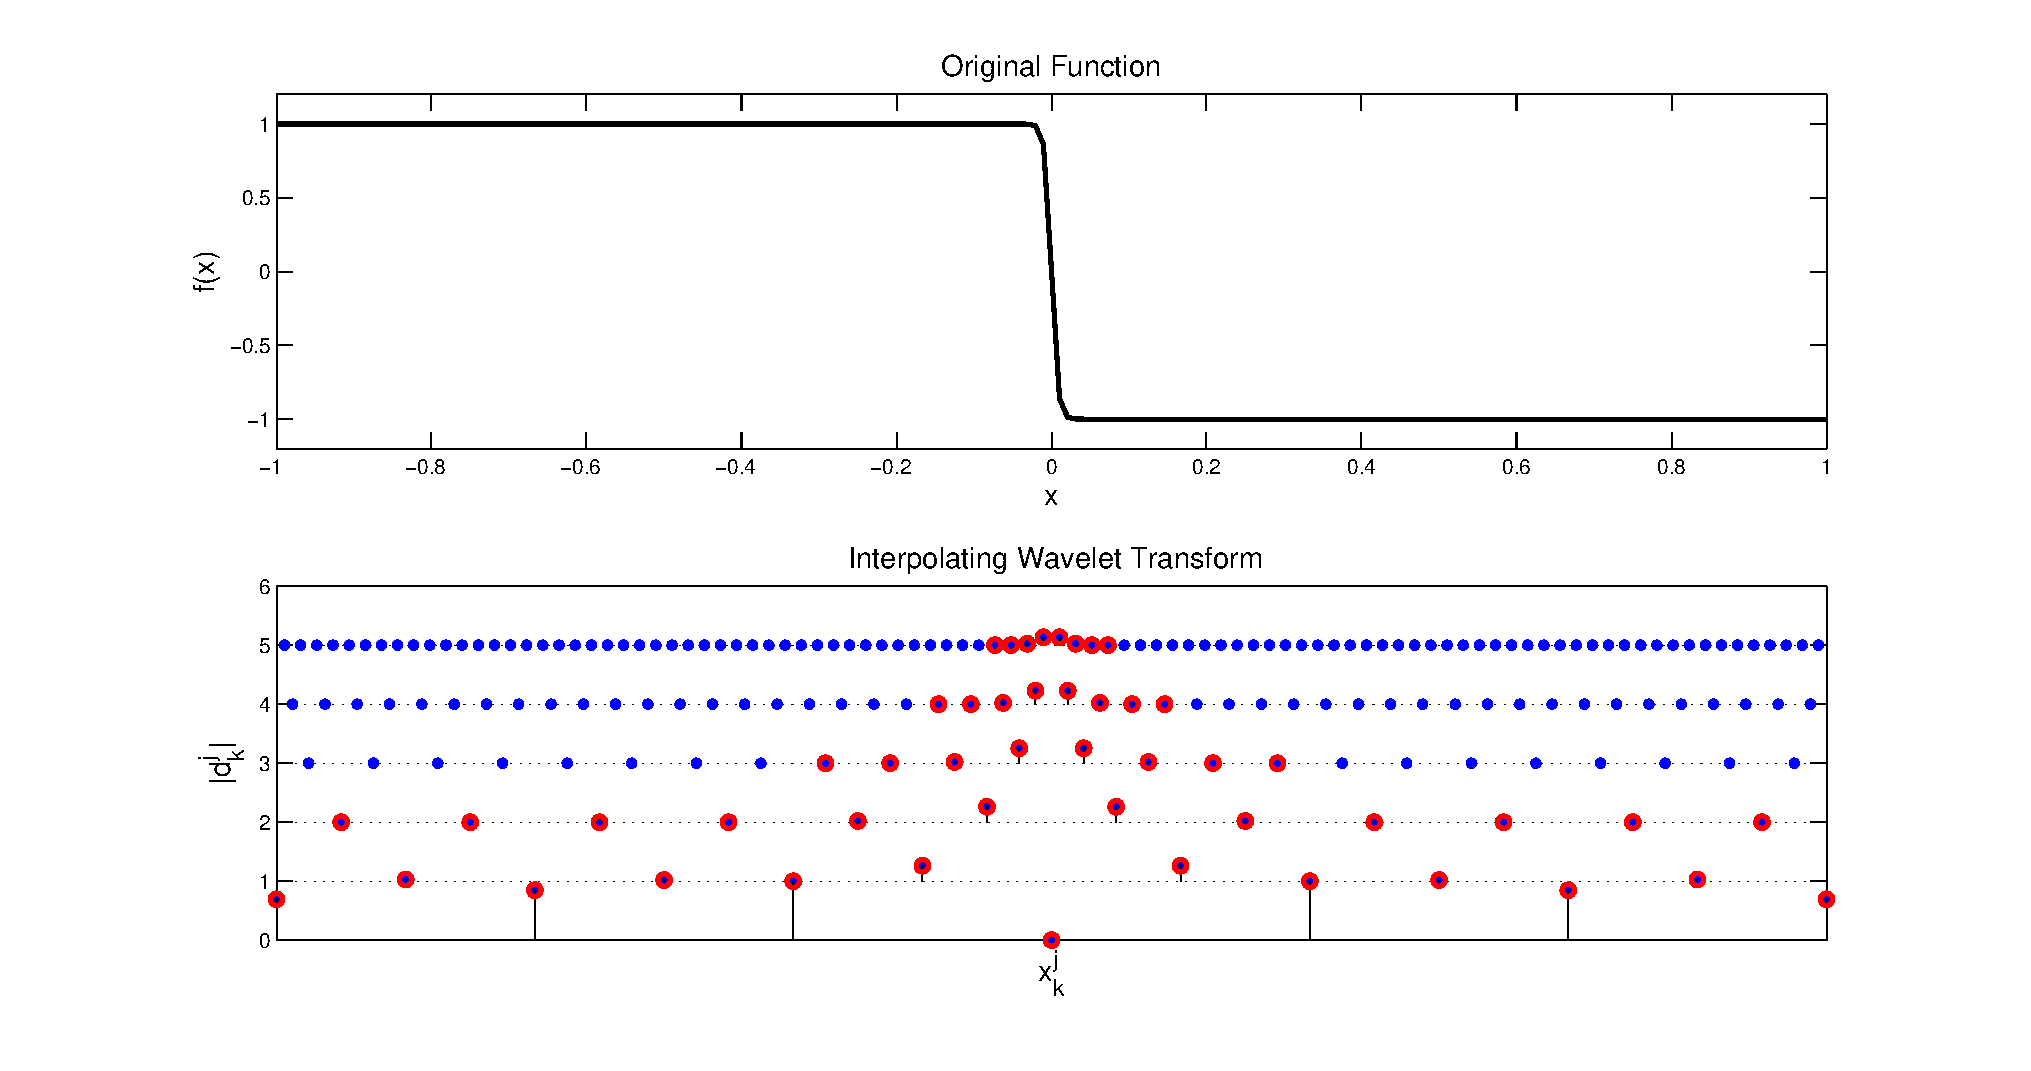
\includegraphics[width=5in]{Images/wavelet}\\
  \caption[1D example of AWCM.]{A one dimensional example of grid adaptation using the Adaptive Wavelet Collocation method.}\label{f:wavelets}
\end{figure}
\end{center}

There are some additional computational costs associated with the use of the adaptive multi-resolution wavelet method.  Currently, the cost per grid point is approximately three to five times greater than the cost of a standard non-adaptive method.  However, in cases of large compressions \cite{05KV} (up to $10^{3}$), the compression greatly outweighs this cost.  There is also some memory savings associated with using adaptive methods, which allows higher resolution simulations to be ran with the same computational resources.  

In summary, the dynamically adaptive wavelet collocation method is an adaptive, variable order method for solving partial differential equations with localized structures that change their location and scale in space and time.  Because the computational grid automatically adapts to the solution (in position and scale), we do not have to know {\it a priori\/} where the  regions of high gradients or structures exist. In related work the dynamically adaptive wavelet collocation method has been combined with the Brinkman penalization method~\cite{kevlahan-vasilyev:2005,kevlahan-ghidaglia:2001} to define solid structures in the domain for the simulation of complex geometry flows.

\section{Brinkman Penalization}

\subsection{Methods for Representing Boundaries with Complex Geometries}

In ocean modeling, one of challenges in how to accurately represent the coastal boundaries and the bathymetry of the ocean floor.  With the inherent complicated geometry that exists, there are two general techniques used mostly commonly.  The first is body-fitted grids, which have been used by fluid dynamics community for some time \cite{82TWM, 90Mavri}.  As mentioned in Section \ref{sec:BackOceanModeling}, the majority of ocean models are using structured or unstructured body-fitted grid methods.  These methods generate grids to conform to the complex boundaries, which can be very expensive.  This makes for easy implementation of boundary conditions, but in order to resolve boundary layers there is a need for a fine resolution near the boundary.  Since most ocean models do not have adaptive or even non-uniform grids, this can be too expensive.  Even for the structured and unstructured meshes that are adaptive and non-uniform, the grid generation and solution interpolation to the new mesh is prohibitively expensive.    

The other approach for representing complex geometries is immersed boundary methods \cite{02Peskin, 02MI}.  These methods work by carrying out simulations on non-body conformal fixed Cartesian grids and then formulated a procedure that imposes immersed boundary effects on the fluid.  It makes for straightforward implementation of solid boundaries of arbitrary complexity.  
 
\subsection{Immersed Boundary Methods for Incompressible Flows}

Immersed boundary methods were originally introduced by Peskins for biomedical applications of flow patterns around heart valves, for incompressible viscous flows \cite{72Peskin}.    In this case, the immersed boundary is modeled as elastic media, which exerts localized forces on the fluids through a modification of the momentum equations.  This was also done for a solid obstacle, where a stiff spring with a restoring force was used instead of the elastic media \cite{00LP}.  This method was then extended, to use a feedback forcing to represent the immersed boundary effects for rigid body problems \cite{93GHS, 96SB}.  The problem with these immersed boundary methods is that they all use an explicit time step.  For these stiff problems, the result is a very restrictive time step.  Additionally, they all use non-adaptive grids, which are very inefficient for high Reynolds number boundary layer flows.  Lastly, there is no mathematical convergence proof for any of these methods.

There are a few other immersed boundary techniques for incompressible viscous flow that use external forces to simulate the immersed boundary.  There is Cartesian grid methods \cite{79PB, 86CSH, 93ZP, 98BA} and ghost-cell methods \cite{03TF}, which directly impose the boundary conditions on the immersed boundary.  

The SUNTANS model from Standford \cite{06FGS} is using immersed boundary methods. 

\subsection{Brinkman Penalization for Incompressible Flows}

Another immersed boundary method is the Brinkman penalization method, originally proposed by Arquis and Caltagirone \cite{84AC}.  It is a volume penalization technique where the boundary conditions are imposed by adding the penalization terms to the momentum equations, similar to the Peskin's immersed boundary methods.  Brinkman penalization works by modeling solid obstacles and boundaries as porous media and setting the parameters associated with the porous media in the limit of a solid body.  There are many benefits to using Brinkman penalization over the other immersed boundary methods.  The first is that it can be used with any numerical method or grid.  Since it only directly modifies the equations, how you solve the equations does not change the method.  Its main advantage is that the error can be estimated rigorously in terms of the penalization parameter \cite{99ABF}.  Lastly, it can be shown that the solutions of the penalized incompressible Navier-Stokes equations strongly converges to the exactly solution as the penalization parameter approaches zero \cite{99Angot}.    

This formulation of Brinkman penalization can be used for the primitive equations, since it is in the same form as the incompressible Navier-Stokes equations.  Figure \ref{f:bpdiagram} shows a schematic of traditional boundary conditions versus Brinkman penalization.

\begin{center}
\begin{figure}[h!]
\centering
  % Requires \usepackage{graphicx}
  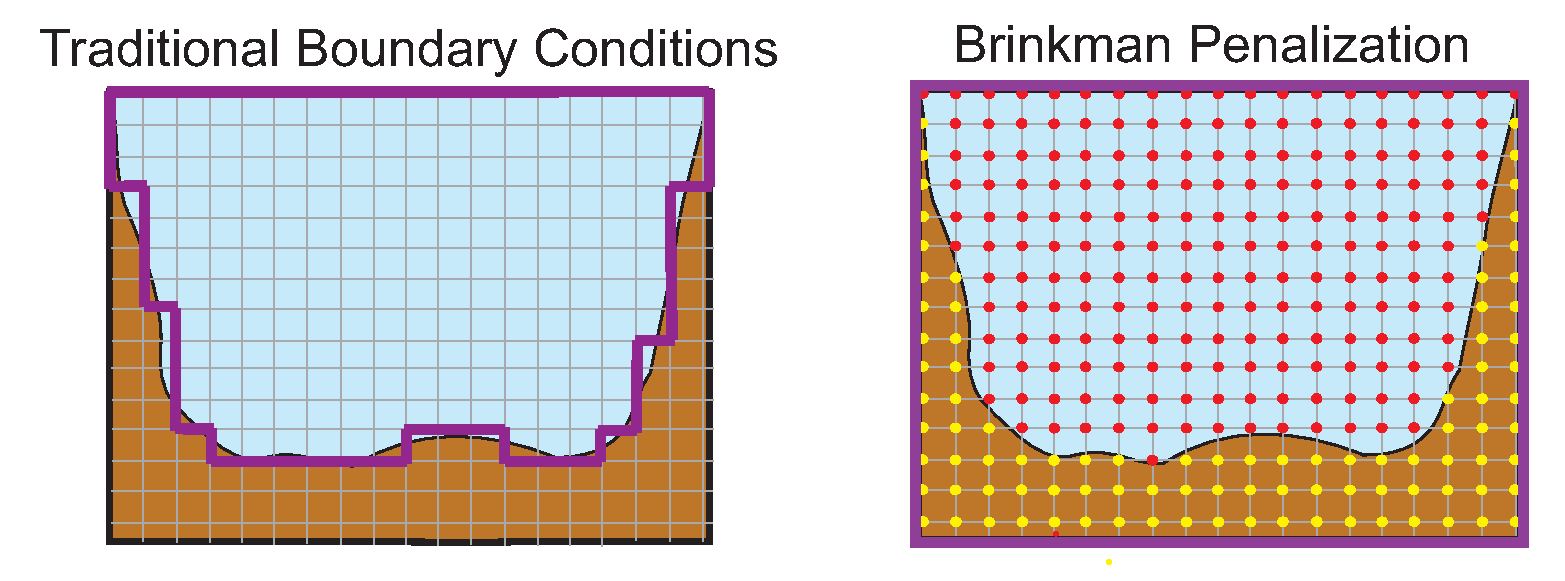
\includegraphics[width=5in]{Images/bpdiagram}\\
  \caption[Traditional boundaries vs. Brinkman penalization]{A schematic of traditional boundary conditions versus brinkman penalization.}\label{f:bpdiagram}
\end{figure}
\end{center}

\subsection{Immersed Boundary Methods for Compressible Flows}

Immersed boundary methods are less popular for compressible viscous flows.  There were some developments with the Cartesian rid method to simulate compressible flows around a circular cylinder and an airfoil at high Reynolds numbers.  In this case, the acoustic wave reflection and transmission at the interface between the fluid and solid was not taken into account, which is critical.  Another technique is the Impedance Mismatch Method, which is used to model the acoutic wave propagation around solid wall boundaries using the non-body conformal cartesian grids.   this method was originally developed by Chung \cite{95Chung} and the later used for linearized acoutic problems with steady mean flows \cite{98CM, 00LM, 00AM}.  This method works by setting a larger characteristic impedance inside the solid obstacle or boundary so that most acoustic waves are reflected by the classical theory of acoustics.  The errors associated with this method are not sufficiently accurate in some cases.  Another drawback is that this method has no one of implementing no-slip boundary conditions or other immersed boundary conditions.  

\subsection{Brinkman Penalization for Compressible Flows}

Brinkman penalization was extended to compressible flow by Liu and Vasilyev \cite{06LV}.  In addition to penalizing the momentum and energy equations as in done the incompressible formulation, the continuity equation for porous media is considered inside obstacles.  Therefore, the penalized porous region acts as a high impedance medium and results in negligible wave transmissions.  The results of the direct numerical simulations were in excellent agreement with the analytical solutions and the numerical simulations verify the accuracy and convergences rates.  

The compressible formulation of Brinkman penalization can be extended to work for the shallow water equations.  The shallow water equations are mathematically equivalent to the compressible gas dynamic equations, for which this formulation was developed.  Further details about the extension are in the following chapters.  

